\documentclass[conference]{IEEEtran}

\usepackage[utf8]{inputenc}
\usepackage[T1]{fontenc}
\usepackage{amsmath,amssymb}
\usepackage{graphicx}
\usepackage{tikz}
\usetikzlibrary{shapes.geometric, arrows.meta, positioning, fit, backgrounds, calc}
\usepackage{booktabs}
\usepackage{multirow}
\usepackage{tabularx}
\usepackage{url}
\usepackage{hyperref}
\usepackage{cite}
\usepackage{balance}
\usepackage{xcolor}
\usepackage{enumitem}
\usepackage{array}

% Compact lists
\setlist{nosep, leftmargin=*}

% TikZ styles
\tikzset{
  block/.style={rectangle, draw, rounded corners, minimum height=0.7cm,
    minimum width=1.8cm, align=center, font=\scriptsize, fill=blue!8},
  decision/.style={diamond, draw, aspect=2.2, align=center,
    font=\scriptsize, fill=yellow!10, inner sep=1pt},
  action/.style={rectangle, draw, rounded corners, minimum height=0.6cm,
    minimum width=1.5cm, align=center, font=\scriptsize, fill=green!10},
  alert/.style={rectangle, draw, rounded corners, minimum height=0.6cm,
    minimum width=1.5cm, align=center, font=\scriptsize, fill=red!10},
  arr/.style={-{Stealth[length=2mm]}, thick},
  phase/.style={rectangle, draw, rounded corners, minimum height=0.8cm,
    minimum width=2.2cm, align=center, font=\small\bfseries, fill=blue!15},
}

\begin{document}

% TITLE & AUTHORS
\title{Extending Kubernetes Self-Healing for Networking Failure}

\author{
  \IEEEauthorblockN{Arpan Gupta,
    Buha Deep Maheshbhai,
    Param Tanna,\\%
    Ramji Purwar,
    Rathod Yuvraj Rajubhai,
    Solanki Viraj Rajeshbhai}
  \IEEEauthorblockA{Indian Institute of Technology Gandhinagar\\
    \{24110051, 24110082, param.tanna,
    ramji.purwar, yuvraj.rathod, viraj.solanki\}@iitgn.ac.in}
}

\maketitle

% I. ABSTRACT
\begin{abstract}
Kubernetes provides robust self-healing for container lifecycle events such as pod crashes and node failures; however, it remains fundamentally blind to network-layer degradation including Container Network Interface (CNI) plugin failures, DNS service disruptions, NetworkPolicy enforcement drift, and silent overlay tunnel breakages. These network failures cause cascading application outages despite all pods appearing healthy to the orchestrator. In this paper, we present our custom Kubernetes operator that continuously monitors and auto-remediates four critical network subsystems: CNI health (Calico), CoreDNS availability, NetworkPolicy dataplane enforcement, and pod-to-pod connectivity. The operator employs a modular \emph{Check~$\to$~Evaluate~$\to$~Remediate} pipeline architecture, where each module independently gathers network telemetry signals, applies threshold-based and triangulation-based failure classification, and executes targeted corrective actions via the Kubernetes API. For connectivity monitoring, we adapt the Pingmesh ring topology to achieve $O(N)$ probe scalability combined with a three-tier triangulation engine for root-cause isolation. The system is driven by a single cluster-scoped Custom Resource Definition (CRD) that exposes configurable detection thresholds and safety guardrails. We validate our operator across Several fault-injection experiments on a multi-node Minikube cluster with Calico CNI, demonstrating automated recovery from CNI agent crashes, IPAM pool exhaustion, DNS latency spikes, corrupted upstream configurations, stale firewall rules, and broken overlay tunnels.
\end{abstract}

% II. INTRODUCTION
\section{Introduction}

\subsection{Background and Motivation}
Kubernetes has emerged as the de facto orchestration platform for containerized microservices~\cite{k8s-docs}. Its built-in self-healing mechanisms-liveness probes, readiness probes, and deployment controllers-effectively handle container-level failures such as process crashes, out-of-memory kills, and node evictions. However, these mechanisms operate strictly at the \emph{container lifecycle} layer and have no visibility into the network data plane.

In production Kubernetes clusters, the network fabric is a complex stack comprising: (i)~a Container Network Interface (CNI) plugin (e.g., Calico, Cilium) that manages IP address allocation, virtual ethernet (veth) interfaces, and inter-node overlay tunnels~\cite{cni-spec, calico-docs}; (ii)~CoreDNS for cluster-internal service discovery and external name resolution~\cite{coredns-docs}; and (iii)~NetworkPolicy resources whose enforcement is delegated to the CNI's dataplane agent (e.g., Calico's Felix daemon) via \texttt{iptables} or eBPF rules.

When any component in this stack degrades-a CNI agent crashes, DNS latency spikes, or an IP-in-IP tunnel interface drops-Kubernetes continues to report pods as \texttt{Running}~(1/1~Ready) and nodes as \texttt{Ready}. Application traffic silently fails with connection timeouts, DNS resolution errors, or unauthorized packet leakage, leading to cascading service disruptions without any automated recovery.

\subsection{Existing Solutions and Their Limitations}

Several tools address aspects of Kubernetes network observability, but none provide continuous, closed-loop self-healing across the full network stack:

\begin{itemize}
  \item \textbf{Native Kubernetes:} DaemonSet controllers restart crashed CNI pods, but Kubernetes does not monitor IPAM capacity, DNS query latency, policy enforcement fidelity, or inter-node tunnel health~\cite{k8s-docs}.
  \item \textbf{Goldpinger~\cite{goldpinger}:} Deploys a full-mesh ping agent across nodes for connectivity visualization but performs no automated remediation and scales at $O(N^2)$.
  \item \textbf{Microsoft Pingmesh~\cite{pingmesh2015}:} Pioneered data-center-scale latency measurement using controller-orchestrated probing but was designed for bare-metal switches, not Kubernetes overlay networks, and does not include remediation logic.
  \item \textbf{NetBouncer~\cite{netbouncer2019}:} Provides active device and link failure localization in data center networks but operates below the Kubernetes abstraction layer.
\end{itemize}

\subsection{Contributions}

This paper makes the following contributions:
\begin{enumerate}
  \item A \textbf{modular operator architecture} with a unified \emph{Check~$\to$~Evaluate~$\to$~Remediate} pipeline that covers four network subsystems: CNI, CoreDNS, NetworkPolicy, and pod-to-pod connectivity.
  \item An \textbf{$O(N)$ Pingmesh-inspired ring probing topology} with three-tier triangulation for root-cause isolation of inter-node and intra-node network failures.
  \item A \textbf{CRD-driven configuration model} with per-module safety guardrails (auto-heal toggles, cooldown windows, escalation limits) enabling both autonomous and audit-only deployment modes.
  \item \textbf{Comprehensive validation} across several fault-injection experiments demonstrating automated recovery from real-world network failure scenarios.
\end{enumerate}

% III. LIMITATIONS OF KUBERNETES SELF-HEALING
\section{Limitations of Kubernetes Network Self-Healing}

Kubernetes was designed to manage container lifecycles, not network infrastructure health. This section identifies four categories of network failures that Kubernetes cannot detect or recover from autonomously.

\subsection{CNI Plugin Failures}
The CNI plugin (e.g., Calico) is responsible for pod IP allocation via IPAM, veth pair creation, and BGP routing mesh establishment~\cite{calico-docs, cni-spec}. When the \texttt{calico-node} DaemonSet agent crashes or becomes unresponsive:
\begin{itemize}
  \item New pods remain stuck in \texttt{ContainerCreating} state indefinitely, as the kubelet cannot invoke the CNI binary to configure the pod's network namespace.
  \item The node may be marked \texttt{NotReady} if the kubelet's network plugin status check fails, but Kubernetes takes no action to restart the CNI agent or recover IP allocations.
  \item IPAM pool exhaustion (all IPs allocated in a subnet) causes all new pod scheduling to fail with \texttt{``No IPs available in pools''}, yet the Kubernetes scheduler has zero awareness of IPAM capacity.
  \item An inadvertently disabled Calico IPPool (\texttt{spec.disabled:~true}) silently blocks all new IP allocations cluster-wide.
\end{itemize}

\subsection{CoreDNS Failures}
CoreDNS provides the foundational DNS resolution service for Kubernetes service discovery~\cite{coredns-docs}. Native Kubernetes manages CoreDNS pod lifecycle but is blind to:
\begin{itemize}
  \item \textbf{Latency degradation:} CPU throttling can spike DNS query round-trip times from $\sim$2\,ms to $>$1000\,ms while pods remain \texttt{Running/Ready}. Kubernetes has no metric for application-layer DNS query duration.
  \item \textbf{Upstream misconfiguration:} Corrupted \texttt{forward} directives in the Corefile ConfigMap break external name resolution while internal \texttt{*.svc.cluster.local} resolution appears healthy.
  \item \textbf{Scale-to-zero:} If an operator or CI script accidentally scales CoreDNS replicas to zero, Kubernetes respects the desired state and leaves cluster DNS completely broken.
\end{itemize}

\subsection{NetworkPolicy Enforcement Drift}
Kubernetes stores NetworkPolicy resources declaratively in etcd but delegates enforcement entirely to the CNI's dataplane agent~\cite{calico-docs}. In Calico, the Felix daemon translates policies into Linux kernel \texttt{iptables}/\texttt{ipset} rules. If Felix crashes or enters \texttt{CrashLoopBackOff}:
\begin{itemize}
  \item The kernel packet-filtering rules freeze in their last-known state.
  \item New policy creations, updates, or deletions are silently ignored by the kernel.
  \item \texttt{kubectl get networkpolicy} continues to show policies as active, creating a false sense of security-traffic that should be blocked remains permitted.
\end{itemize}

\subsection{Pod-to-Pod Connectivity Failures}
Pod-to-pod communication traverses virtual interfaces (veth pairs), host bridges, and overlay tunnels (IPIP/VXLAN)~\cite{calico-docs}. Kubernetes readiness probes only verify that a local process responds on a port-they do not validate that the virtual network fabric can deliver cross-node or intra-node traffic. When a veth interface is administratively downed, an IP-in-IP tunnel crashes, or iptables \texttt{FORWARD} rules are corrupted:
\begin{itemize}
  \item Pods remain \texttt{Running (1/1 Ready)} on both the source and destination nodes.
  \item Application requests time out silently with no Kubernetes event or alert.
  \item Kubernetes has no mechanism for active network path probing or topology-aware failure detection.
\end{itemize}

% IV. SYSTEM ARCHITECTURE AND DESIGN
\section{System Architecture and Design}

\subsection{Operator and Custom Resource Definition}

Our operator is implemented as a Kubernetes operator following the controller pattern~\cite{kubebuilder, controller-runtime}. The system is governed by a single cluster-scoped Custom Resource Definition (CRD), \texttt{NetworkRemediation} (API version \texttt{v1alpha1}), which serves as the declarative specification for all monitoring and remediation behavior.

The CRD specification is decomposed into four independent module configurations: \texttt{CNISpec}, \texttt{CoreDNSSpec}, \texttt{NetworkPolicySpec}, and \texttt{PodConnectivitySpec}. Each module specification exposes: (i)~an \texttt{enabled} toggle for independent activation; (ii)~detection thresholds and intervals; and (iii)~safety guardrails controlling whether the operator may perform mutating actions or operate in audit-only mode.

Table~\ref{tab:crd-spec} summarizes the key configurable parameters for each module.

\begin{table}[t]
\centering
\caption{CRD Module Configuration Summary}
\label{tab:crd-spec}
\renewcommand{\arraystretch}{1.15}
\setlength{\tabcolsep}{3pt}
\footnotesize
\begin{tabular}{@{}l l l@{}}
\toprule
\textbf{Module} & \textbf{Key Parameters} & \textbf{Defaults} \\
\midrule
\multirow{3}{*}{CNI} & \texttt{stuckPodThresholdSec} & 60\,s \\
                     & \texttt{ipamUsageThreshold\%} & 80\% \\
                     & \texttt{calicoNodeLabel} & \texttt{k8s-app=calico-node} \\
\midrule
\multirow{4}{*}{CoreDNS} & \texttt{expectedReplicas} & 2 \\
                         & \texttt{latencyThresholdMs} & 150\,ms \\
                         & \texttt{autoHealReplicas} & true \\
                         & \texttt{autoHealConfigMap} & true \\
\midrule
\multirow{2}{*}{NetworkPolicy} & \texttt{autoHeal} & true \\
                               & \texttt{cooldownSeconds} & 60\,s \\
\midrule
\multirow{6}{*}{\shortstack[l]{Pod\\Connectivity}} & \texttt{targetNamespace} & \texttt{default} \\
                                                    & \texttt{consecutiveFailThreshold} & 3 \\
                                                    & \texttt{autoRemediationEnabled} & true \\
                                                    & \texttt{maxRestartAttempts} & 2 \\
\bottomrule
\end{tabular}
\end{table}

\subsection{Three-Phase Pipeline Architecture}

The core design principle of our operator is the separation of concerns across three distinct operational phases, implemented as a common \texttt{Module} interface that all four network subsystem modules adhere to:

\begin{enumerate}
  \item \textbf{Check Phase (Signal Gathering):} Collects raw network telemetry-pod statuses, DaemonSet health, IPAM allocations, DNS query latencies, active probe results-without making any decisions.
  \item \textbf{Evaluate Phase (Failure Classification):} Analyzes gathered signals against configurable thresholds to classify severity (\texttt{info}, \texttt{warning}, \texttt{critical}) and determine whether automated remediation is warranted. This phase prevents false positives by requiring sustained threshold breaches.
  \item \textbf{Remediate Phase (Corrective Action):} Executes the minimum necessary Kubernetes API mutations to restore network health-pod deletions (triggering DaemonSet respawns), deployment scaling, ConfigMap patches, node taints, or workload evictions.
\end{enumerate}

Fig.~\ref{fig:pipeline} illustrates the three-phase pipeline within the reconciliation loop.

\begin{figure}[t]
\centering
\resizebox{0.78\columnwidth}{!}{%
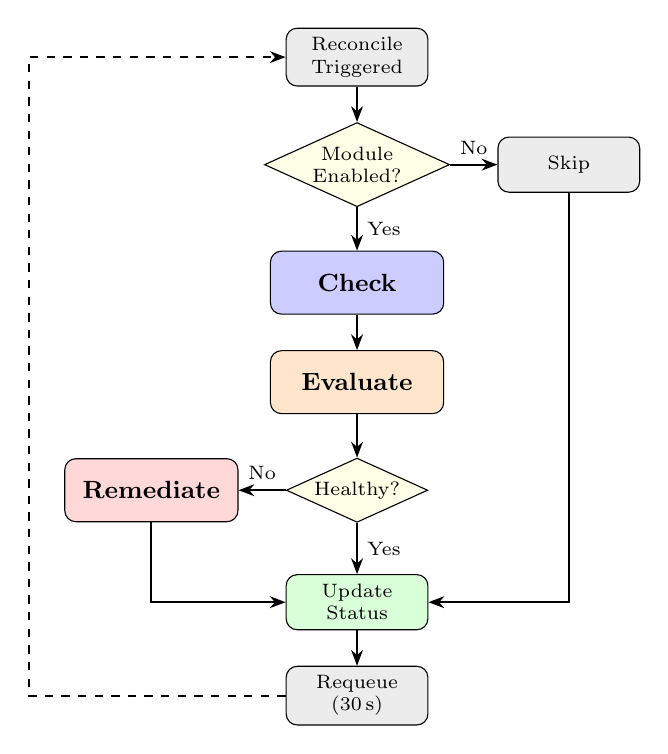
\begin{tikzpicture}[node distance=0.45cm and 0.5cm]
  \node[block, fill=gray!15] (trigger) {Reconcile\\Triggered};
  \node[decision, below=0.45cm of trigger] (enabled) {Module\\Enabled?};
  \node[block, fill=gray!15, right=0.6cm of enabled] (skip) {Skip};
  \node[phase, fill=blue!20, below=0.55cm of enabled] (check) {Check};
  \node[phase, fill=orange!20, below=0.45cm of check] (eval) {Evaluate};
  \node[decision, below=0.55cm of eval] (healthy) {Healthy?};
  \node[phase, fill=red!15, left=0.6cm of healthy] (rem) {Remediate};
  \node[block, fill=green!15, below=0.65cm of healthy] (status) {Update\\Status};
  \node[block, fill=gray!15, below=0.45cm of status] (requeue) {Requeue\\(30\,s)};

  \coordinate (loopleft) at ($(rem.west)+(-0.45cm, 0)$);
  
  \draw[arr] (trigger) -- (enabled);
  \draw[arr] (enabled) -- node[above, font=\scriptsize] {No} (skip);
  \draw[arr] (enabled) -- node[right, font=\scriptsize] {Yes} (check);
  \draw[arr] (check) -- (eval);
  \draw[arr] (eval) -- (healthy);
  \draw[arr] (healthy) -- node[right, font=\scriptsize] {Yes} (status);
  \draw[arr] (healthy) -- node[above, font=\scriptsize] {No} (rem);
  \draw[arr] (rem.south) |- (status.west);
  \draw[arr] (skip.south) |- (status.east);
  \draw[arr] (status) -- (requeue);
  \draw[arr, dashed] (requeue.west) -- (requeue.west -| loopleft) -- (trigger.west -| loopleft) -- (trigger.west);

\end{tikzpicture}%
}% end resizebox
\caption{Check $\to$ Evaluate $\to$ Remediate pipeline within the reconciliation loop. Each module runs this pipeline independently every 30\,s.}
\label{fig:pipeline}
\end{figure}

\subsection{Dispatcher and Module Registration}

The central reconciler acts as a \emph{dispatcher}. On each reconciliation cycle, it: (i)~fetches the \texttt{NetworkRemediation} custom resource; (ii)~iterates through all registered modules; (iii)~skips disabled modules; (iv)~executes the Check~$\to$~Evaluate~$\to$~Remediate pipeline for each enabled module; (v)~updates per-module status fields in the CR; and (vi)~requeues for periodic re-check after 30 seconds.

This design ensures complete modularity-each network subsystem module operates independently, can be developed separately, and can be toggled on or off at runtime without affecting other modules. Fig.~\ref{fig:architecture} shows the overall system architecture.

\begin{figure}[t]
\centering
\resizebox{0.85\columnwidth}{!}{%
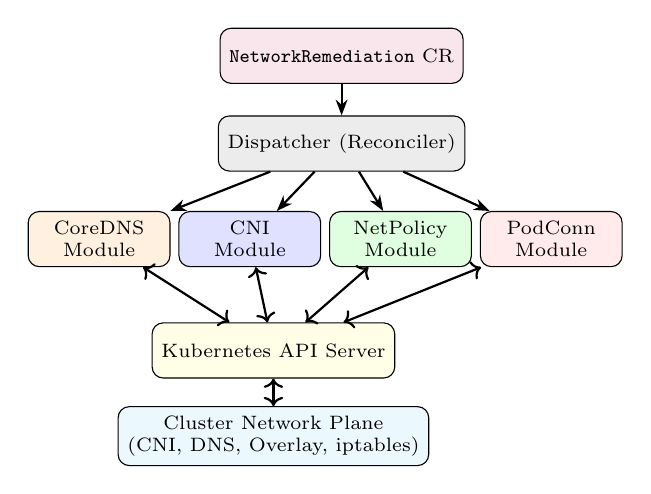
\begin{tikzpicture}[node distance=0.3cm and 0.2cm]
  % CR
  \node[block, fill=purple!10, minimum width=2.8cm] (cr) {\texttt{NetworkRemediation} CR};
  
  % Dispatcher
  \node[block, fill=gray!15, minimum width=2.8cm, below=0.4cm of cr] (disp) {Dispatcher (Reconciler)};
  
  % Modules
  \node[block, fill=orange!12, below left=0.5cm and 0.6cm of disp] (dns) {CoreDNS\\Module};
  \node[block, fill=blue!12, right=0.1cm of dns] (cni) {CNI\\Module};
  \node[block, fill=green!12, right=0.1cm of cni] (np) {NetPolicy\\Module};
  \node[block, fill=red!8, right=0.1cm of np] (pc) {PodConn\\Module};
  
  % Kubernetes API
  \node[block, fill=yellow!10, minimum width=3cm, below=0.7cm of cni, xshift=0.3cm] (api) {Kubernetes API Server};
  
  % Network plane
  \node[block, fill=cyan!8, minimum width=3cm, below=0.35cm of api] (net) {Cluster Network Plane\\(CNI, DNS, Overlay, iptables)};
  
  \draw[arr] (cr) -- (disp);
  \draw[arr] (disp) -- (dns);
  \draw[arr] (disp) -- (cni);
  \draw[arr] (disp) -- (np);
  \draw[arr] (disp) -- (pc);
  \draw[arr, <->] (dns) -- (api);
  \draw[arr, <->] (cni) -- (api);
  \draw[arr, <->] (np) -- (api);
  \draw[arr, <->] (pc) -- (api);
  \draw[arr, <->] (api) -- (net);
\end{tikzpicture}%
}% end resizebox
\caption{System architecture. The dispatcher reads the CRD and runs each module's pipeline. Modules interact with the Kubernetes API for telemetry and remediation.}
\label{fig:architecture}
\end{figure}


% V. DETECTION AND REMEDIATION POLICIES
\section{Detection and Remediation Policies}

This section describes the detection signals, evaluation heuristics, and remediation actions for each network subsystem module.

\subsection{CNI Module}

\subsubsection{Detection Signals}
The CNI module continuously gathers four categories of signals:
\begin{enumerate}
  \item \textbf{DaemonSet Health:} Compares \texttt{desiredNumberScheduled} against \texttt{numberReady} on the \texttt{calico-node} DaemonSet. Any mismatch triggers enumeration of unready pods.
  \item \textbf{Stuck Workload Pods:} Scans all cluster pods in \texttt{Pending} phase with empty \texttt{podIP}. Pods exceeding the configurable stuck threshold (default: 60\,s) are flagged.
  \item \textbf{CNI Event Correlation:} Queries Kubernetes warning events for \texttt{FailedCreatePodSandBox} messages containing CNI/IPAM error signatures.
  \item \textbf{IPAM Capacity:} Queries Calico \texttt{IPPool} and \texttt{IPAMBlock} CRDs to detect disabled pools (\texttt{spec.disabled:~true}) and exhausted blocks (100\% utilization).
\end{enumerate}

\subsubsection{Evaluation Heuristics}
The evaluator applies a strict priority ordering to avoid conflating symptoms with root causes:
\begin{enumerate}
  \item \emph{Unready calico-node agents} $\to$ \texttt{critical} severity, action: restart agents.
  \item \emph{Disabled IPPool with stuck pods} $\to$ \texttt{critical}, action: re-enable pool.
  \item \emph{Stuck pods with CNI errors} $\to$ \texttt{critical}, action: evict stuck pods.
  \item \emph{IPAM usage $\geq$ threshold} $\to$ \texttt{warning}, no disruptive action (log only).
\end{enumerate}

\subsubsection{Remediation Actions}
Three targeted remediation branches are executed based on the evaluation:
\begin{itemize}
  \item \textbf{Restart CNI Agents:} Deletes unready \texttt{calico-node} pods; the DaemonSet controller immediately respawns fresh agents that re-establish BGP routing and veth interfaces.
  \item \textbf{Re-enable IPPool:} Patches \texttt{spec.disabled} to \texttt{false} on affected Calico IPPools, unblocking IP allocations.
  \item \textbf{Evict Stuck Pods:} Deletes workload pods stranded in \texttt{ContainerCreating} to force rescheduling with clean network namespace initialization.
\end{itemize}

\subsection{CoreDNS Module}

\subsubsection{Detection Signals}
The CoreDNS module monitors five aspects of DNS service health:
\begin{enumerate}
  \item \textbf{Replica Availability:} Inspects the \texttt{coredns} Deployment for \texttt{availableReplicas} vs. \texttt{expectedReplicas} (default: 2).
  \item \textbf{Pod Readiness:} Identifies pods in \texttt{CrashLoopBackOff}, \texttt{Error}, or unready states.
  \item \textbf{DNS Query Latency:} Queries Prometheus for average request duration over a 1-minute window:
  \begin{equation}
    \text{Latency} = \frac{\texttt{rate(sum[1m])}}{\texttt{rate(count[1m])}}
    \label{eq:latency}
  \end{equation}
  \item \textbf{Upstream Configuration:} Parses the Corefile ConfigMap to validate \texttt{forward} directive targets against known-bad subnets (RFC~5737~\cite{rfc5737}: \texttt{192.0.2.0/24}, \texttt{198.51.100.0/24}, \texttt{203.0.113.0/24}).
  \item \textbf{Resource Starvation:} Detects CPU limits $\leq$5\,m that cause latency spikes despite pods appearing healthy.
\end{enumerate}

\subsubsection{Remediation Actions}
\begin{itemize}
  \item \textbf{Scale Recovery:} Patches the CoreDNS Deployment replicas back to \texttt{expectedReplicas}.
  \item \textbf{Pod Restart:} Deletes unready/crashlooping pods to trigger clean respawns.
  \item \textbf{ConfigMap Repair:} Replaces corrupted \texttt{forward} targets with fallback servers (default: \texttt{/etc/resolv.conf}, \texttt{8.8.8.8}) and triggers a rolling restart.
  \item \textbf{Resource Restoration:} Resets CPU limits to baseline (100\,m) when throttling is detected.
\end{itemize}

Each remediation type is gated by independent safety toggles (\texttt{autoHealReplicas}, \texttt{autoHealConfigMap}) and a 30\,s cooldown window to prevent restart thrashing.

\subsection{NetworkPolicy Module}

\subsubsection{Detection Signals}
The NetworkPolicy module targets the \emph{control-plane-to-dataplane disconnect} described in Section~III-C. It audits all \texttt{calico-node} pods in \texttt{kube-system} for:
\begin{itemize}
  \item Pod phase $\neq$ \texttt{Running}
  \item Container readiness $=$ \texttt{false}
  \item Container restart count $\geq$~3
  \item Container state: \texttt{CrashLoopBackOff} or \texttt{Error}
\end{itemize}

Any pod matching these criteria indicates that the Felix enforcement agent is not actively programming kernel packet-filtering rules, leaving the dataplane in a stale state.

\subsubsection{Remediation Actions}
When unhealthy enforcement agents are detected and \texttt{autoHeal} is enabled, the operator deletes the degraded \texttt{calico-node} pod. The DaemonSet controller respawns a fresh pod, and on startup, Felix reads all declared policies from the Kubernetes API and programs \texttt{iptables}/\texttt{ipset} chains from scratch, clearing stale rules. A configurable cooldown (default: 60\,s) rate-limits consecutive restarts to prevent control plane churn.

\subsection{Pod-to-Pod Connectivity Module}

\subsubsection{Probing Topology}
We adapt the Pingmesh~\cite{pingmesh2015} approach to Kubernetes by establishing a deterministic ring topology across $N$ worker nodes. Nodes are sorted lexicographically and connected as:
\begin{equation}
  \text{Forward: } Node_i \to Node_{(i+1) \bmod N}
\end{equation}
\begin{equation}
  \text{Reverse: } Node_i \to Node_{(i-1+N) \bmod N} \quad (N \geq 3)
\end{equation}

This yields exactly $2N$ inter-node probes, achieving $O(N)$ scalability versus the $O(N^2)$ cost of full-mesh probing. Each node additionally undergoes an $O(1)$ intra-node canary validation to verify local veth, bridge, and iptables FORWARD chain integrity.

\subsubsection{Three-Tier Triangulation}
The evaluate phase employs a three-tier pattern analysis engine to isolate root causes and prevent false remediation:

\noindent\textbf{Tier~1 - Local CNI Validation:} If a node's local probe fails but its system anchors (gateway, CoreDNS) are reachable, the root cause is isolated to the local CNI subsystem (dropped veth, corrupted eBPF map).

\noindent\textbf{Tier~2 - Inter-Node Triangulation:} When $Node_A \not\to Node_B$, the operator checks if $Node_C \to Node_B$ succeeds. If all peers fail to reach $Node_B$, the ingress network stack on $Node_B$ is declared dead. If only $Node_A$ fails, the issue is an asymmetric path/tunnel drop.

\noindent\textbf{Tier~3 - Anchor Corroboration:} For small clusters ($N < 3$) where triangulation is insufficient, probes against high-availability anchors (default gateway, \texttt{kube-apiserver}) disambiguate host-level versus tunnel-level failures.

Fig.~\ref{fig:triangulation} illustrates the three-tier triangulation decision tree.

\begin{figure}[t]
\centering
\resizebox{0.95\columnwidth}{!}{%
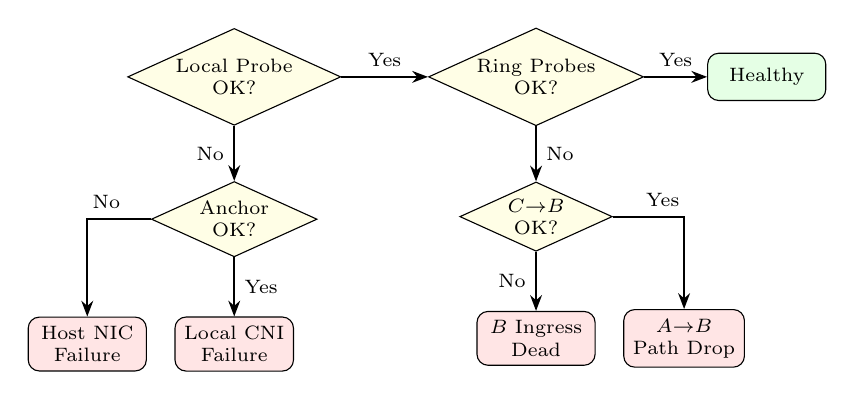
\begin{tikzpicture}[every node/.style={font=\scriptsize}]
  % Top row
  \node[decision] (local) {Local Probe\\OK?};
  \node[decision, right=1.1cm of local] (ring) {Ring Probes\\OK?};
  \node[action, right=0.8cm of ring] (ok) {Healthy};
  
  % Middle row
  \node[decision, below=0.7cm of local] (anchor1) {Anchor\\OK?};
  \node[decision, below=0.7cm of ring] (tri) {$C{\to}B$\\OK?};
  
  % Bottom row (4 mutually exclusive failure outcomes)
  \node[alert, below=0.75cm of anchor1] (localcni) {Local CNI\\Failure};
  \node[alert, left=0.35cm of localcni] (blackhole) {Host NIC\\Failure};
  
  \node[alert, below=0.75cm of tri] (ingress) {$B$ Ingress\\Dead};
  \node[alert, right=0.35cm of ingress] (path) {$A{\to}B$\\Path Drop};
  
  % Connections - Top and Middle
  \draw[arr] (local) -- node[above, font=\scriptsize] {Yes} (ring);
  \draw[arr] (local) -- node[left, font=\scriptsize] {No} (anchor1);
  \draw[arr] (ring) -- node[above, font=\scriptsize] {Yes} (ok);
  \draw[arr] (ring) -- node[right, font=\scriptsize] {No} (tri);
  
  % Connections - Left branch (Anchor)
  \draw[arr] (anchor1) -- node[right, font=\scriptsize] {Yes} (localcni);
  \draw[arr] (anchor1.west) -| node[above, font=\scriptsize, pos=0.35] {No} (blackhole.north);
  
  % Connections - Right branch (Triangulation)
  \draw[arr] (tri) -- node[left, font=\scriptsize] {No} (ingress);
  \draw[arr] (tri.east) -| node[above, font=\scriptsize, pos=0.35] {Yes} (path.north);
\end{tikzpicture}%
}% end resizebox
\caption{Three-tier triangulation decision tree for root-cause isolation of connectivity failures.}
\label{fig:triangulation}
\end{figure}

\subsubsection{Hierarchical Remediation Policy}
Remediation escalates through three tiers of increasing blast radius:

\noindent\textbf{Tier~1 - CNI Agent Restart:} Deletes the \texttt{calico-node} pod on the affected node. The DaemonSet respawns the agent, which flushes stale routing tables, resets tunnel interfaces (\texttt{tunl0}, \texttt{vxlan.calico}), and rebinds veth pairs. Limited to \texttt{maxRestartAttempts} (default: 2).

\noindent\textbf{Tier~2 - Node Taint and Cordon:} If CNI restarts fail, the operator patches the Kubernetes Node resource with a \texttt{network-degraded:NoSchedule} taint and sets \texttt{spec.unschedulable = true}, preventing new workload placement on the degraded host.

\noindent\textbf{Tier~3 - Workload Drain:} As a last resort, the operator safely evicts all non-DaemonSet pods using the Kubernetes Eviction API, respecting PodDisruptionBudgets. Workloads are rescheduled onto healthy nodes by their parent controllers.


% VI. EXPERIMENTAL SETUP AND VALIDATION
\section{Experimental Setup and Validation}

\subsection{Cluster Environment}
All experiments are conducted on a multi-node Minikube cluster configured as shown in Table~\ref{tab:env-spec}.

\begin{table}[t]
\centering
\caption{Experimental Environment Specifications}
\label{tab:env-spec}
\renewcommand{\arraystretch}{1.1}
\setlength{\tabcolsep}{4pt}
\footnotesize
\begin{tabular}{@{}l l@{}}
\toprule
\textbf{Component} & \textbf{Configuration} \\
\midrule
Cluster & Minikube (Docker driver), 2 nodes \\
Resources per Node & 2 vCPUs, 4096\,MB RAM \\
CNI Plugin & Calico (calico-node DaemonSet) \\
DNS Server & CoreDNS (2 replicas, kube-system) \\
Kubernetes Version & v1.31+ \\
Operator Framework & Kubebuilder v4.15+, Go 1.24+ \\
Test Workloads & backend-api, frontend-probe, dns-checker \\
Replicas per Workload & 2 (spread across both nodes) \\
\bottomrule
\end{tabular}
\end{table}

\subsection{Fault Injection Methodology}
Each experiment follows a three-phase methodology: (i)~establish a healthy cluster baseline; (ii)~inject a specific network fault and observe native Kubernetes behavior (no operator); (iii)~enable the operator and verify automated detection and recovery.

Table~\ref{tab:experiments} summarizes the fault-injection experiments conducted across all four modules.

\begin{table}[t]
\centering
\caption{Summary of Fault-Injection Experiments}
\label{tab:experiments}
\renewcommand{\arraystretch}{1.1}
\setlength{\tabcolsep}{3pt}
\footnotesize
\begin{tabular}{@{}l p{4.2cm} c@{}}
\toprule
\textbf{Module} & \textbf{Fault Injected} & \textbf{Healed} \\
\midrule
CNI & calico-node agent crash & \checkmark \\
CNI & IPAM pool exhaustion & \checkmark \\
CNI & IPPool disabled & \checkmark \\
CoreDNS & Scale replicas to zero & \checkmark \\
CoreDNS & CPU throttle ($\leq$5\,m) & \checkmark \\
CoreDNS & Corrupted upstream forward & \checkmark \\
NetPolicy & Felix agent crash & \checkmark \\
PodConn & veth interface down & \checkmark \\
PodConn & IPIP tunnel crash & \checkmark \\
PodConn & iptables FORWARD DROP & \checkmark \\
PodConn & Inter-node overlay break & \checkmark \\
\bottomrule
\end{tabular}
\end{table}

\subsection{Validation Results}
Across all experiments, the operator successfully detected the injected network failure within the first reconciliation cycle (30\,s) and executed the appropriate remediation action. Key observations include:
\begin{itemize}
  \item \textbf{CNI recovery:} Unready calico-node pods were restarted within 30--60\,s, with BGP routing mesh convergence completing within an additional 10--15\,s.
  \item \textbf{DNS restoration:} Scale-to-zero recovery restored full DNS availability within one reconciliation cycle. Corrupted upstream configurations were repaired and pods rolling-restarted within 45\,s.
  \item \textbf{Policy resynchronization:} Crashed Felix agents were replaced within 30\,s; kernel iptables rules were fully reprogrammed by the respawned agent within 5--10\,s of pod startup.
  \item \textbf{Connectivity recovery:} The Pingmesh ring detected overlay tunnel failures within a single probe interval (10\,s), and CNI agent restarts restored cross-node connectivity within 30--60\,s.
\end{itemize}


% VII. CONCLUSION AND FUTURE SCOPE
\section{Conclusion and Future Scope}

\subsection{Conclusion}
We presented our custom Kubernetes operator that extends the platform's self-healing capabilities to the network data plane. By implementing a modular Check~$\to$~Evaluate~$\to$~Remediate pipeline across four critical network subsystems-CNI, CoreDNS, NetworkPolicy enforcement, and pod-to-pod connectivity-our operator detects and auto-remediates network failures that are invisible to native Kubernetes mechanisms.

The operator's $O(N)$ Pingmesh-inspired ring probing topology and three-tier triangulation engine enable scalable, accurate root-cause isolation of connectivity failures without the $O(N^2)$ overhead of full-mesh probing. The CRD-driven configuration model provides operators with fine-grained control over detection thresholds, safety guardrails, and remediation escalation, supporting both fully autonomous and audit-only deployment modes.

Validation across all fault-injection experiments confirmed that our operator achieves automated recovery from diverse real-world network failures including CNI agent crashes, IPAM exhaustion, DNS degradation, stale firewall rules, and broken overlay tunnels, typically within 30--60\,s of fault occurrence.

\subsection{Future Work}
Several directions remain for future development:
\begin{itemize}
  \item \textbf{Alertmanager Integration:} Connecting operator events to Prometheus Alertmanager for external notification channels (PagerDuty, Slack, email).
  \item \textbf{eBPF-Based Probing:} Replacing TCP/ICMP probes with eBPF kernel-level probes for deeper, lower-overhead CNI introspection.
  \item \textbf{Machine Learning Anomaly Detection:} Training time-series models on DNS latency and probe telemetry to detect subtle degradation patterns before threshold breaches.
  \item \textbf{Multi-Cluster Federation:} Extending the operator to monitor and heal cross-cluster networking in federated Kubernetes environments.
  \item \textbf{Helm Chart and OLM Packaging:} Publishing the operator via Helm charts and the Operator Lifecycle Manager catalog for production deployment.
\end{itemize}

% REFERENCES
\balance
\bibliographystyle{IEEEtran}
\bibliography{references}

\end{document}
